\documentclass[a4paper]{article}

\usepackage[english]{babel}
\usepackage[utf8]{inputenc}
\usepackage{amsmath}
\usepackage{graphicx}
\usepackage{float}
\restylefloat{table}

\title{Improvements and extensions on a Social Simulation.}

\author{prive}

\date{\today}

\begin{document}

\maketitle

\begin{abstract}
	In this paper we describe a simulation of pedestrians crossing a busy road. In particular, we study the effects of higher (or otherwise 'more effective') fines and higher police presence on the likelihood of people crossing the road when the pedestrian light is red. Our aim was to incorporate the influence people have on each other. We found that [1-2 zinnen samenvatting van resultaten hier].
\end{abstract}

\clearpage
\tableofcontents
\clearpage

\section{Existing model}
The existing model for this social simulation was written in NetLogo. The goal of the simulation was to discover what the influence of police presence is on the number of red light walkers. In the model, pedestrians made their decision to walk through a red light based on the following factors:
\begin{itemize}
\item Pedestrians exert \textit{peer pressure} on other pedestrians,
\item Pedestrians gain valuable time by crossing a red light,
\item Pedestrians make a loss when they get caught.
\end{itemize}

\subsection{Design}
The world consists out of 33 by 33 patches and wraps around. A road with two traffic lights, one for the pedestrians and one for the cars, is located in this world. Within the simulation there are two types of agents: pedestrians and cars. The pedestrians move horizontally through the world and due to the wrap around keep crossing the road. The cars on the other hand move along the vertical axis. The intersection of the pedestrians and the cars forms the crossing place.

Pedestrians are divided in three so called 'walker types'. The first one is the $cautious$ type. A cautious pedestrian will only cross the road if the traffic light is green and no car is approaching. The second walker type is the $reckless$ type. A reckless person will cross the road whenever it sees an opportunity, regardless of the traffic light. The final walker type is the $adaptive$ type. An adaptive person can either behave like a cautious person or a reckless person depending on its past experiences and the amount of profit the pedestrian expects to gain by walking through red.

\subsection{Simulation}
\label{sec:initialsim}
For the simulation, the following parameters were used for all experiments: The fine was set to $\$250$, the number of pedestrians to $50$ and the pedestrians' green time was $20$ ticks. Additionally, the following experiment-specific parameters were used:\\

\begin{tabular}{ r | l | l }
  Exp. & Cars & Car green time (ticks) \\
  \hline
  1 &  0 & 100 \\
  2 & 10 & 100 \\
  3 & 50 & 100 \\
  4 &  0 & 20  \\
  5 & 10 & 20  \\
  6 & 50 & 20  \\
\end{tabular}\\

Running the simulation for $100 000$ ticks, the results were as follows:
\begin{table}[H]
\centering
\begin{tabular}{ l | c c c c }
  Police Presence Prob. & 0\% & 33\% & 66\% & 100\% \\ 
  \hline
  Experiment 1 & 3.92 & 2.40 & 0 & 0  \\
  Experiment 2 & 0.15 & 0.03 & 0 & 0  \\
  Experiment 3 & 0    & 0    & 0 & 0  \\
  Experiment 4 & 0.37 & 0    & 0 & 0  \\
  Experiment 5 & 0.15 & 0    & 0 & 0  \\
  Experiment 6 & 0    & 0    & 0 & 0  \\
\end{tabular}
\caption{Average number of times an adaptive 
pedestrian walks through a red light.}
\end{table}

\clearpage

\section{Changes and their immediate effects}
In this section we summarize the changes we made to the model, why, and how they affected the simulation.

\subsection{Viewing Distance}
We introduced a 'viewing range' for agents, where they would only be able to look ahead a fixed amount of $patches$ for oncoming cars. In the existing simulation, pedestrians would look ahead from their current y position to the y position of the traffic light (top right of the road). This meant different pedestrians looked at bigger portions of the road than others. For example, in figure \ref{ABlabel}, the pedestrian marked $A$ would only look ahead three patches, while the pedestrians marked $B$ would look ahead the entire road.

\begin{figure}[H]
\centering
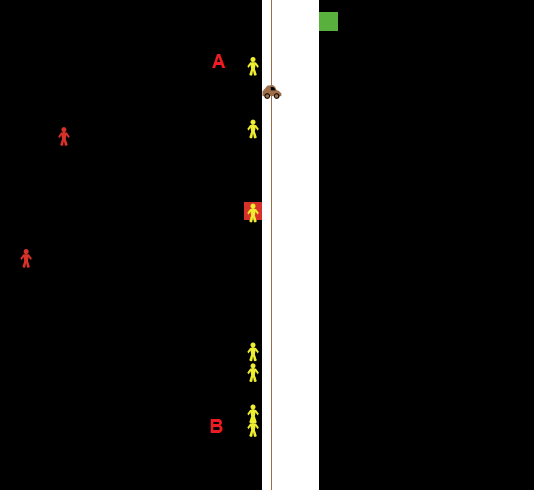
\includegraphics[width=.75\textwidth]{socsim1.png}
\caption{Visualization of the simulation.}
\label{ABlabel}
\end{figure}

If a pedestrian would spot cars on the portion of the road it was watching, it would refuse to cross. As a result, even a moderate amount of cars resulted in pedestrians located at the bottom of the road not crossing when the light was red, regardless of their 'type'.

Additionally, pedestrians standing close to the traffic light would only look ahead a few patches, not noticing cars that might be approaching just behind the traffic light.

\subsubsection{Implementation and influences on the simulation}
The pedestrian's logic was rewritten to look ahead a fixed number of patches rather than looking ahead until the traffic light. This 'viewing range' would also wrap around the world, meaning the viewing range of pedestrians standing near the top of the road also covered part of the bottom of the road. This ensures that all pedestrians regardless of their vertical position in the world observed an equally sized portion of the road.

The area between the bottom of the road and the traffic light was 24 patches high. Consequently, the average viewing range of a pedestrian was about 12 patches.

To quantify the influence of this change on the simulation and its results, we set the viewing range to 8 (picked arbitrarily for testing), and ran the simulation with the exact same parameters as in chapter \ref{sec:initialsim}. The results were:

\begin{table}[H]
\centering
\begin{tabular}{ l | c c c c }
  Police Presence Prob. & 0\% & 33\% & 66\% & 100\% \\ 
  \hline
  Experiment 1 & 3.46 & 2.31 & 0 & 0  \\
  Experiment 2 & 1.83 & 1.31 & 0 & 0  \\
  Experiment 3 & 0.54 & 0.27 & 0 & 0  \\
  Experiment 4 & 0.46 & 0    & 0 & 0  \\
  Experiment 5 & 0.50 & 0    & 0 & 0  \\
  Experiment 6 & 0.13 & 0    & 0 & 0  \\
\end{tabular}
\caption{Average number of times an adaptive 
pedestrian walks through a red light.}
\end{table}

The results for experiments 1 and 4, where no cars were on the road, did not change much, as expected. Interestingly, the results for experiments 2, 3, 5 and 6, when more cars were on the road, increased noticably. 

\subsection{More advanced model}
The movement logic of the pedestrians was adapted to arrive at the road in a more spread out fashion, rather than all at rougly the same moment.

When looking at the old model pedestrians would move across the world in a vertical band along the x-axis all clustered together. This was countered by the slightly random movement speed of the pedestrians, but since the movement was evaluated each tick the resulting difference was minimal. Ultimately all the agents would arrive at the traffic light within a few ticks of each other.

Another aspect that was changed was the constant y-coordinate of the pedestrians. During a simulations the pedestrians would remain on the same vertical coordinate. Varying this was needed to counter the same agent crossing an optimal spot multiple times. After implementing the viewing distance it became clear that crossing the road at the bottom was more profitable since it takes a while before the cars to enter the viewing range of the bottom most pedestrians when the cars' traffic light turns green.
Since it is important for this simulation to reuse the same agents, recreating pedestrians anew wasn't an option.

\subsubsection{Implementation}
The implementation of the advanced model was done by creating a "waiting zone" in the world. The first column of patches are colored blue in the simulation to visualize this zone. Once a pedestrian enters this zone it will get a random number of ticks it has to wait and its y-coordinate is randomized.
After the wait time is over the pedestrian will continue its normal movement routine.

\subsection{Counting methods}
Some of the figures extracted from the old simulation were meaningless. Many of the percentages were calculated by dividing the number of pedestrians that performed a certain task, say walking through a red light, by the total number of pedestrians in the simulation. This was done without taking into account that some pedestrians weren't even near the road or that the counted pedestrians were already counted.

This became an even bigger problem after the waiting zone was introduced. It allowed for an even bigger gap between the total number of people and the actual number of people crossing the road or near the road.

\subsubsection{Implementation}
The implementation is done by counting the number of pedestrians per cycle and using that as denominator for calculating the percentages. Every pedestrian approaching the road will be counted towards the total of the current cycle. A new cycle starts whenever the pedestrians' traffic light goes red.


\subsection{Crossing Chance}
The crossing behaviour of adaptive people was changed to be based on chance instead of being based on a fixed treshold.

In the old model adaptive pedestrians would cross when there was no car approaching and a certain treshold was reached. The effect of the police enforcement was determined by the value of the fine. Fined people would not cross at a red light for a certain amount of ticks corresponding to the height of the fine. However we believe that this does not approximate human decison making very well. Decisons are not always rational and based on fixed rules and values. To better approximate the decision whether or not to cross the road at a red light we use a probability. 

The chance to cross at a certain moment is found by looking at past experiences and circumstancial factors, so called push and pull factors. Those influence either increasing or decreasing the probability a pedestrian would cross. This implementation allows multiple factors to be easily added to the model.

One thing we wanted to look at was how a fine effects the people's behaviour. There are studies that researched the correlation between the height of a fine and its effect, but they don't show a clear correlation and contradiction conclusions can be found. This study ......$1$ looked at the the effects of a higher fine on drunk driving incidents, did not show that higher fines really did have greater effectiveness. To avoid this we set the fine in $effectiveness$ instead of a certain money value and leave the implementation of the fine out of the model. 

We found that personal experience plays a big role in decision making, as is shown in ..$2$... The paper shows that personal experience of getting a fine for returning a rented movie to late, effects the chance of bringing it late again the next time. The effect of the experience however diminshes over time. But experience is not only experiencing something yourself, like getting fined, but seeing and hearing about it is also an experience. Although the forms may convey the same information they do no have the same effect on a decision is remarked it the paper. That's why we implemented the three forms to effect the decison of the adaptives, the effect however diminisches over time and the chance goes back to its original value.

\subsubsection{Implementation}

The way we implemented our new model for crossing is by replacing the cooldown value of the existing model by two new variables. The first variable which is set randomly at the beginning 

\clearpage

\section{Simulation}
\subsection{Setup}
The figures we are interested in are the actual amount of adaptive pedestrians that cross the road during a red light and the likeliness that they walk through a red light. During the simulation the following parameters will stay the same:
\begin{itemize}
\item Pedestrian green time: $25$ ticks
\item Car green time: $50$ ticks
\item Experiencing weight: 1.0
\item Seeing weight: 0.4
\item Hearing weight: 0.1
\end{itemize}
These values aren't based on any real world values, but turned out to exhibit behaviour that allows all implemented features to be used. If the pedestrians' light is red there are still gaps in the approaching cars for pedestrians to cross the road. Furthermore there are moments that only a few pedestrians are next to road and moments there are plenty allowing both influenced and uninfluenced probabilities of crossing. 

Each simulation will be run for $10000$ ticks. At the end the average percentage of adaptive walking through a red light and the average probability of the adaptive are recorded. The variables that are varied during the experiments are the police appearance probability and the effectiveness of the fine. For the police probability the values $25$, $50$, $75$ and $100$ will be chosen and for the fine $20$, $40$, $60$, $80$ and $100$. These twenty experiments are repeated for different number of pedestrians and number of cars. These will vary from high and low where high is 50 for pedestrian and 80 for cars, low is 20 for pedestrians and 40 for cars.

\clearpage
\subsection{Results 20 pedestrians and 40 cars}
In this simulation the number of pedestrians and the number of cars are kept low. This means that the influence pedestrians have on each other will have less effect. Also there are more openings in the oncoming car traffic for pedestrians to cross the road.

\begin{table}[H]
\centering
\begin{tabular}{ l | c c c c }
  Fine\slash Prob. & 25\% & 50\% & 75\% & 100\% \\ 
  \hline
  20\%  & 30.2 / 37.0 & 22.1 / 25.9 & 20.9 / 19.3 & 21.1 / 16.7  \\
  40\%  & 22.0 / 31.1 & 18.0 / 26.3 & 17.7 / 20.7 & 17.3 / 16.5  \\
  60\%  & 20.6 / 31.4 & 18.8 / 27.4 & 16.0 / 20.7 & 14.3 / 17.7  \\
  80\%  & 21.5 / 23.4 & 16.3 / 28.2 & 14.5 / 20.9 & 12.9 / 17.5  \\
  100\% & 24.8 / 27.1 & 16.5 / 29.9 & 13.8 / 22.4 & 11.0 / 16.2  \\
\end{tabular}
\end{table}

\begin{table}[H]
\centering
\begin{tabular}{ l | c c c c }
  Fine\slash Prob. & 25\% & 50\% & 75\% & 100\% \\ 
  \hline
  20\%  & 1.2 & 1.2 & 0.9 & 0.8  \\
  40\%  & 1.4 & 1.5 & 1.2 & 1.0  \\
  60\%  & 1.5 & 1.5 & 1.3 & 1.2  \\
  80\%  & 1.5 & 1.7 & 1.4 & 1.4  \\
  100\% & 1.9 & 1.8 & 1.6 & 1.5  \\
\end{tabular}
\end{table}

\subsection{Results 50 pedestrians and 40 cars}
In this simulation the number of pedestrians is increased.

\begin{table}[H]
\centering
\begin{tabular}{ l | c c c c }
  Fine\slash Prob. & 25\% & 50\% & 75\% & 100\% \\ 
  \hline
  20\%  & 25.5 / 35.2 & 24.5 / 27.9 & 21.5 / 18.3 & 20.9 / 12.7  \\
  40\%  & 25.8 / 30.6 & 20.5 / 30.2 & 16.8 / 18.9 & 16.0 / 13.3  \\
  60\%  & 20.7 / 31.8 & 17.1 / 23.9 & 14.2 / 16.8 & 13.4 / 11.9  \\
  80\%  & 21.5 / 31.2 & 14.3 / 21.4 & 12.2 / 17.2 & 11.5 / 11.0  \\
  100\% & 17.6 / 32.2 & 12.8 / 25.4 & 11.1 / 18.2 & 10.8 / 10.7  \\
\end{tabular}
\end{table}

\begin{table}[H]
\centering
\begin{tabular}{ l | c c c c }
  Fine\slash Prob. & 25\% & 50\% & 75\% & 100\% \\ 
  \hline
  20\%  & 1.4 & 1.1 & 0.9 & 0.6  \\
  40\%  & 1.2 & 1.5 & 1.1 & 0.8  \\
  60\%  & 1.5 & 1.4 & 1.2 & 0.9  \\
  80\%  & 1.5 & 1.5 & 1.4 & 1.0  \\
  100\% & 1.8 & 2.0 & 1.6 & 1.0  \\
\end{tabular}
\end{table}

\clearpage
\subsection{Results 20 pedestrians and 80 cars}
In this simulation the number of pedestrians is kept low while the number of cars is increased. During the cars' green time there will be less gaps for the pedestrians to slip through. This means the most likely moment for them to walk through red is at the start of the pedestrians' red light.

\begin{table}[H]
\centering
\begin{tabular}{ l | c c c c }
  Fine\slash Prob. & 25\% & 50\% & 75\% & 100\% \\ 
  \hline
  20\%  & 26.0 / 29.9 & 26.8 / 22.6 & 21.9 / 19.9 & 22.3 / 14.0  \\
  40\%  & 25.6 / 29.9 & 23.2 / 29.6 & 19.2 / 19.0 & 18.3 / 13.9  \\
  60\%  & 22.8 / 31.1 & 15.4 / 25.0 & 16.3 / 18.2 & 12.9 / 13.2  \\
  80\%  & 18.8 / 31.2 & 15.4 / 22.7 & 15.8 / 21.9 & 12.3 / 12.6  \\
  100\% & 19.5 / 29.2 & 14.0 / 23.8 & 15.9 / 16.7 & 11.2 / 13.0  \\
\end{tabular}
\end{table}

\begin{table}[H]
\centering
\begin{tabular}{ l | c c c c }
  Fine\slash Prob. & 25\% & 50\% & 75\% & 100\% \\ 
  \hline
  20\%  & 1.2 & 0.8 & 0.9 & 0.6  \\
  40\%  & 1.2 & 1.3 & 1.0 & 0.8  \\
  60\%  & 1.4 & 1.6 & 1.1 & 1.0  \\
  80\%  & 1.7 & 1.5 & 1.4 & 1.0  \\
  100\% & 1.5 & 1.7 & 1.0 & 1.2  \\
\end{tabular}
\end{table}

\subsection{Results 50 pedestrians and 80 cars}
In this simulation both the number of pedestrians and the number of cars are high. This simulation represents a busy road, both for cars and pedestrians.

\begin{table}[H]
\centering
\begin{tabular}{ l | c c c c }
  Fine\slash Prob. & 25\% & 50\% & 75\% & 100\% \\ 
  \hline
  20\%  & 27.4 / 30.7 & 23.3 / 23.3 & 20.0 / 17.5 & 20.5 / 11.1  \\
  40\%  & 24.5 / 32.1 & 20.8 / 27.2 & 16.7 / 17.3 & 16.9 / 11.5  \\
  60\%  & 20.7 / 24.4 & 15.7 / 21.6 & 15.5 / 16.6 & 13.2 / 10.2  \\
  80\%  & 22.3 / 29.0 & 14.1 / 24.9 & 14.6 / 15.8 & 11.7 / 10.0  \\
  100\% & 19.2 / 29.6 & 14.3 / 21.5 & 11.2 / 16.3 &  9.7 /  9.3  \\
\end{tabular}
\end{table}

\begin{table}[H]
\centering
\begin{tabular}{ l | c c c c }
  Fine\slash Prob. & 25\% & 50\% & 75\% & 100\% \\ 
  \hline
  20\%  & 1.1 & 1.0 & 0.9 & 0.5  \\
  40\%  & 1.3 & 1.3 & 1.0 & 0.7  \\
  60\%  & 1.2 & 1.4 & 1.1 & 0.8  \\
  80\%  & 1.3 & 1.8 & 1.1 & 0.9  \\
  100\% & 1.5 & 1.5 & 1.5 & 1.0  \\
\end{tabular}
\end{table}

\clearpage

\section{Conclusion}
When looking at the result it becomes clear that increasing the effectiveness without increasing the police presence will reduce the chance of adaptive walking through red, but the actual percentage of those adaptive walking through red stays roughly the same. This is most likely due to peer pressure. Since getting caught is unlikely, but once you get caught it is effective, the probability will vary greatly among the adaptive. When an adaptive with a high probability walks through red it will increase the chance of all adaptives to do the same. An adaptive with an average probability crosses the road due to the first one and gives a boots to the other adaptive with a lower probability.

On the other hand, only increasing the police presence but not the effectiveness of the fine will bring the actual percentage of adaptive crossing closer to the average probability of the adaptive crossing. The probability of the adaptive crossing falls slightly when increasing the presence.

So increasing the fine results in a lower red walking chance, but leaves the actual percentage the same. Increasing the police presence lowers the actual percentage of red walking and leaves the chance roughly the same. One would assume that increasing both would result in the best possible outcome. But looking at the results that isn't the case...

\clearpage

\begin{thebibliography}{3}

	\bibitem{name} description

\end{thebibliography}

\end{document}
